\section{METODOLOGI}

% Ubah konten-konten berikut sesuai dengan isi dari metodologi

\subsection{Tools Aplikasi Yang Digunakan}

Sistem ini dibuat pada \emph{operating system} Linux. Untuk dapat
berjalan, sistem ini membutuhkan:

\subsection{Metamask}
Metamask adalah crypto wallet yang biasanya digunakan untuk keperluan development. Crypto wallet ini
akan sangat membantu dalam proses pengembangan. Terdapat banyak fitur-fitur seperti multi-account yang mempermudah proses pengembangan.

\subsection{Remix IDE}
Remix IDE merupakan IDE yang memudahkan kita untuk proses development, deployment, dan membuat smart contract di Ethereum.

\subsection{Ethereum}
Ethereum adalah blockchain opensource dengan fitur smart contract. Fitur smart contract inilah yang akan digunakan untuk 
melakukan sharing data pemutar musik.


\subsubsection{Golang}
Menggunakan golang sebagai bahasa pemrograman untuk web server. Untuk servernya akan menggunakan library Echo. Library Geth
digunakan untuk keperluan mengakses API ethereum pada Golang, Kubo digunakan untuk menghubungkan golang dengan IPFS.

\subsubsection{Docker}
Aplikasi yang bersifat open source yang berfungsi se-
bagai wadah/container untuk mengepak/memasukkan sebuah
software secara lengkap.

\subsubsection{InterPlanetary File System (IPFS )}
Protokol dan peer to
peer network untuk distribusi konten yang cepat, terdistribusi
dan mudah disatukan yang kompatibel untuk semua tipe data
seperti gambar, stream video, database terdistribusi.

\subsection{Metodologi Penelitian}

\begin{figure} [ht] \centering
  % Nama dari file gambar yang diinputkan
  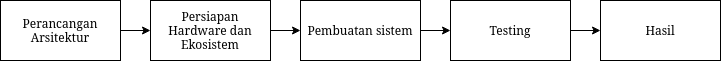
\includegraphics[scale=0.55]{gambar/diagram_blok_metodologi.png}
  % Keterangan gambar yang diinputkan
  \caption{Diagram Blok Metodologi}
  % Label referensi dari gambar yang diinputkan
  \label{fig:Blueprint}
\end{figure}

\subsubsection{Perancangan Arsitektur}
Proses perancangan dari arsiktektur sistem yang meliputi IPFS, server, dan blockchain.

\subsubsection{Persiapan Ekosistem}
Proses penyiapan program-program yang dibutuhkan untuk proses pengembangan sistem.

\subsubsection{Pembuatan sistem}
Proses pembuatan sistem yang meliputi pembuatan platform blockchain, server serta file system

\subsubsection{Testing dan Integrasi}'
Proses melakukan testing \emph{trial and error} untuk pengujian kestabilan sistem serta perbaikan dari sisi performa dan \emph{bug fixing}

\subsubsection{Hasil}
Apabila sistem sudah berjalan dan terintegrasi dengan lancar maka proses selanjutnya adalah pelaporan dalam pembukuan tugas akhir.
